%--------------------------------------------------------------------%
%
% Berkas utama templat LaTeX.
%
% author Petra Barus, Peb Ruswono Aryan, Faris Rizki Ekananda
%
%--------------------------------------------------------------------%
%
% Berkas ini berisi struktur utama dokumen LaTeX yang akan dibuat.
%
%--------------------------------------------------------------------%

\documentclass[bahasa, 12pt, a4paper, onecolumn, oneside, final]{report}

\hyphenpenalty=100000
\tolerance=10000


%-------------------------------------------------------------------%
%
% Konfigurasi dokumen LaTeX untuk laporan tesis IF ITB
%
% @author Petra Novandi
%
%-------------------------------------------------------------------%
%
% Berkas asli berasal dari Steven Lolong
%
%-------------------------------------------------------------------%

% Ukuran kertas
\special{papersize=210mm,297mm}

% Setting margin
\usepackage[top=2cm,bottom=2cm,left=4cm,right=3cm]{geometry}

% Math package
\usepackage{mathptmx}

% 4th Sectioning
\usepackage{titlesec}
\newcommand{\subsubsubsection}[1]{\paragraph{#1}\mbox{}\\}

\titleformat{\subsubsubsection}
{\normalfont\normalsize\bfseries}{\theparagraph}{1em}{}
\titleformat*{\section}{\normalsize\bfseries}
\titleformat*{\subsection}{\normalsize\bfseries}
\titlespacing*{\subsubsubsection}
{0pt}{3.25ex plus 1ex minus .2ex}{1.5ex plus .2ex}

% Judul bahasa Indonesia
\usepackage[bahasa]{babel}

% Format citation
\usepackage[utf8]{inputenc}
\usepackage[style=apa,backend=biber]{biblatex}
\usepackage{longtable}
\usepackage{graphicx}
\usepackage{subfig}
\usepackage{titling}
\usepackage{booktabs}
\usepackage{tabularx}
\usepackage{blindtext}
% \usepackage{sectsty}
\usepackage{chngcntr}
\usepackage{etoolbox}
\usepackage{array}
\usepackage{float}
\usepackage[hidelinks]{hyperref}       % Package untuk link di daftar isi. Ubah jadi \usepackage[hidelinks]{hyperref} apabila ingin menghilangkan kotak merah disekitar link
\usepackage{titletoc}       % Package Format judul di toc
\usepackage{tocbibind}      % Package untuk masukkan toc, lot, lof ke Daftar Isi
\usepackage{scrwfile}       % Package untuk membuat Daftar Lampiran dari toc
\usepackage{parskip}
\usepackage{afterpage}
\usepackage{relsize}
\usepackage{xcolor, colortbl}
\usepackage{setspace}
\usepackage{listings}
\usepackage{csquotes}
\usepackage{multirow}
\usepackage{enumitem}
\usepackage{amsmath}
\usepackage{makecell}
\usepackage{ragged2e}

\graphicspath{{resources/}}   % letak direktori penyimpanan gambar

% Setting daftar lampiran
\newcommand*{\lopname}{DAFTAR LAMPIRAN}
\TOCclone[\lopname]{toc}{atoc}
\addtocontents{atoc}{\protect\value{tocdepth}=-1}
\newcommand\listofappendices{
  \cleardoublepage
  \phantomsection
  \listofatoc
  \addcontentsline{toc}{chapter}{\lopname}
}

\newcommand*\savedtocdepth{}
\AtBeginDocument{%
  \edef\savedtocdepth{\the\value{tocdepth}}%
}

\let\originalappendix\appendix
\renewcommand\appendix{%
  \originalappendix
  \cleardoublepage
  \addtocontents{toc}{\protect\value{tocdepth}=-1}%
  \addtocontents{atoc}{\protect\value{tocdepth}=\savedtocdepth}%

  \titlecontents{chapter}
  [0pt]
  {\bfseries}
  {Lampiran \thecontentslabel.\quad}
  {}
  {\hfill\contentspage}

  \titleformat{\chapter}[block]
  {\bfseries}
  {\chaptertitlename\ \thechapter.\quad}{0pt}
  {\bfseries}
}

% Hilangkan titik pada toc
\makeatletter
\renewcommand{\@dotsep}{1}
\makeatother

% Setel title pada chapter-chapter di toc, lof, lot
\titlecontents{chapter}
[0pt]
{\bfseries}
{\MakeUppercase{Bab} \thecontentslabel\quad\uppercase}
{}
{\mdseries\titlerule*[0.35em]{.}\bfseries\contentspage}
\titlecontents{figure}
[0pt]
{}
{Gambar \thecontentslabel.\quad}
{}
{\mdseries\titlerule*[0.35em]{.}\bfseries\contentspage}
\titlecontents{table}
[0pt]
{}
{Tabel \thecontentslabel.\quad}
{}
{\mdseries\titlerule*[0.35em]{.}\bfseries\contentspage}

% Masukin Daftar Pustaka ke toc
\let\originalprintbibliography\printbibliography
\renewcommand\printbibliography{%
  \phantomsection
  \cleardoublepage
  \originalprintbibliography
  \addcontentsline{toc}{chapter}{\bibname}
}

% Line satu setengah spasi
\renewcommand{\baselinestretch}{1.5}

% Setting judul
% \chapterfont{\centering \large}
\titleformat{\chapter}[display]
{\Large\centering\bfseries}
{\chaptertitlename\ \thechapter}{0pt}
{\Large\bfseries\uppercase}

% Setting nomor pada subbsubsubbab
\setcounter{secnumdepth}{4}

\makeatletter

\makeatother

% Counter untuk figure dan table.
\counterwithin{figure}{chapter}
\counterwithin{table}{chapter}

% Define blank page
\newcommand*{\blankpage}{\afterpage{\null\newpage}}

% Translate autoref into Indonesian
\renewcommand*{\equationautorefname}{Persamaan}%
\renewcommand*{\footnoteautorefname}{catatan kaki}%
\renewcommand*{\itemautorefname}{item}%
\renewcommand*{\figureautorefname}{Gambar}%
\renewcommand*{\tableautorefname}{Tabel}%
\renewcommand*{\partautorefname}{Bagian}%
\renewcommand*{\appendixautorefname}{Lampiran}%
\renewcommand*{\chapterautorefname}{Bab}%
\renewcommand*{\sectionautorefname}{Subbab}%
\renewcommand*{\subsectionautorefname}{Subsubbab}%
\renewcommand*{\subsubsectionautorefname}{Subsubsubbab}%
\renewcommand*{\paragraphautorefname}{paragraf}%
\renewcommand*{\subparagraphautorefname}{subparagraf}%
\renewcommand*{\FancyVerbLineautorefname}{garis}%
\renewcommand*{\theoremautorefname}{Teorema}%
\renewcommand*{\pageautorefname}{halaman}%

% Format to ignore underflow hbadness
\hbadness=99999

% Redefine \cite for Name (Year)
\DeclareCiteCommand{\cite}
{\usebibmacro{prenote}} % Optional prenote
{\printnames{labelname}\space(\printfield{year})} % Name (Year)
{\multicitedelim} % Separator for multiple citations
{\usebibmacro{postnote}} % Optional postnote
% %--------------------------------------------------------------------%
%
% Hypenation untuk Bahasa Indonesia
%
% @author Petra Barus
%
%--------------------------------------------------------------------%
%
% Secara otomatis LaTeX dapat langsung memenggal kata dalam dokumen,
% tapi sering kali terdapat kesalahan dalam pemenggalan kata. Untuk
% memperbaiki kesalahan pemenggalan kata tertentu, cara pemenggalan
% kata tersebut dapat ditambahkan pada dokumen ini. Pemenggalan
% dilakukan dengan menambahkan karakter '-' pada suku kata yang
% perlu dipisahkan.
%
% Contoh pemenggalan kata 'analisa' dilakukan dengan 'a-na-li-sa'
%
%--------------------------------------------------------------------%

\hypenation {
	% A
	%
	a-na-li-sa
	a-pli-ka-si

	% B
	%
	be-be-ra-pa
	ber-ge-rak

	% C
	%
	ca-ri

	% D
	%
	da-e-rah
	di-nya-ta-kan
	de-fi-ni-si

	% E
	%
	e-ner-gi
	eks-klu-sif

	% F
	%
	fa-si-li-tas

	% G
	%
	ga-bung-an

	% H
	%
	ha-lang-an

	% I
	% 
	i-nduk

	% J
	%
	ka-me-ra
	kua-li-tas

	% K
	%

	% L
	%

	% M
	%

	% N
	%

	% O
	%

	% P
	%

	% Q
	%

	% R
	%

	% S
	%

	% T
	% 

	% U
	%

	% V
	%

	% W
	%

	% X
	%

	% Y
	% 

	% Z
	%
}


\makeatletter

\makeatother

\addbibresource{references.bib}

\begin{document}

%Basic configuration
\title{Pembangunan \textit{Dataset Trace} I/O NFS dengan Beban Kerja Pelatihan Pembelajaran Mendalam}
\date{}
\author{
    Bintang Dwi Marthen \\
    NIM : 13521144
}

\pagenumbering{roman}
\setcounter{page}{1}

\clearpage
\pagestyle{empty}

\begin{center}
    \smallskip
    
    \Large \bfseries \MakeUppercase{\thetitle}
    \vfill
    
    \Large Laporan Tugas Akhir
    \vfill
    
    \large Disusun sebagai syarat kelulusan tingkat sarjana
    \vfill
    
    \large Oleh
    
    \Large \theauthor
    
    \vfill
    \begin{figure}[h]
        \centering
        
\includegraphics[width=0.15\textwidth]{cover-ganesha.jpg}
    \end{figure}
    \vfill
    
    \large
    \uppercase{
        Program Studi Teknik Informatika \\
        Sekolah Teknik Elektro \& Informatika \\
        Institut Teknologi Bandung
    }
    
    Juni 2025
    
\end{center}

\clearpage

\clearpage
\pagestyle{empty}

\begin{center}
    \smallskip
    
    \Large \bfseries \MakeUppercase{\thetitle}
    \vfill
    
    \Large Laporan Tugas Akhir
    \vfill
    
    \large Oleh
    
    \Large \theauthor
    
    \large Program Studi Teknik Informatika \\
    
    \normalsize \normalfont
    Sekolah Teknik Elektro dan Informatika \\
    Institut Teknologi Bandung \\
    
    \vfill
    \normalsize \normalfont
    Bandung, xx Juni 2025 \\
    Mengetahui,
    
    \vspace{0.5cm}
    Pembimbing,
    
    \vfill
    \underline{Achmad Imam Kistijantoro, S.T., M.Sc., Ph.D.} \\
    NIP. 197308092006041001
    
\end{center}
\clearpage
 % 1 PEMBIMBING PAKAI INI
% \clearpage
\pagestyle{empty}

\begin{center}
    \smallskip

    \Large \bfseries \MakeUppercase{\thetitle}
    \vfill

    \Large Laporan Tugas Akhir I
    \vfill

    \large Oleh

    \Large \theauthor

    \large Program Studi Teknik Informatika \\

    \normalsize \normalfont
    Sekolah Teknik Elektro dan Informatika \\
    Institut Teknologi Bandung

    \vfill
    \normalsize \normalfont
    Bandung, 21 Oktober 2021 \\
    Mengetahui,

    \vspace{0.5cm}
    \setlength{\tabcolsep}{12pt}
    \begin{tabular}{c@{\hskip 0.5in}c}
        Pembimbing I,                           & Pembimbing II,                           \\
                                                &                                          \\
                                                &                                          \\
                                                &                                          \\
                                                &                                          \\
        \underline{Nama dan Gelar Pembimbing I} & \underline{Nama dan Gelar Pembimbing II} \\
        NIP. 123456789                          & NIP. 123456789                           \\
    \end{tabular}

\end{center}
\clearpage
 % 2 PEMBIMBING PAKAI INI
\chapter*{Lembar Pernyataan}

Dengan ini saya menyatakan bahwa:

\begin{enumerate}

    \item Pengerjaan dan penulisan Laporan Tugas Akhir ini dilakukan tanpa menggunakan bantuan yang tidak dibenarkan.
    \item Segala bentuk kutipan dan acuan terhadap tulisan orang lain yang digunakan di dalam penyusunan laporan tugas akhir ini telah dituliskan dengan baik dan benar.
    \item Laporan Tugas Akhir ini belum pernah diajukan pada program pendidikan di perguruan tinggi mana pun.

\end{enumerate}

Jika terbukti melanggar hal-hal di atas, saya bersedia dikenakan sanksi sesuai dengan Peraturan Akademik dan Kemahasiswaan Institut Teknologi Bandung bagian Penegakan Norma Akademik dan Kemahasiswaan khususnya Pasal 2.1 dan Pasal 2.2.
\vspace{15mm}

Bandung, xx Juni 2025 \\
Bintang Dwi Marthen \\
NIM 13521144


\pagestyle{plain}

\clearpage
\chapter*{ABSTRAK}
\addcontentsline{toc}{chapter}{Abstrak}

%taruh abstrak bahasa indonesia di sini
\blindtext
\clearpage
% \clearpage
\chapter*{Abstract}
\addcontentsline{toc}{chapter}{Abstract}

%put your abstract here
\blindtext

\clearpage
\chapter*{Kata Pengantar}
\addcontentsline{toc}{chapter}{Kata Pengantar}

Gunakan bagian ini untuk memberikan ucapan terima kasih kepada semua pihak yang secara langsung atau tidak langsung membantu penyelesaian tugas akhir, termasuk pemberi beasiswa jika ada. Utamakan untuk memberikan ucapan terima kasih kepada tim pembimbing tugas akhir dan staf pengajar atau pihak program studi, bahkan sebelum mengucapkan terima kasih kepada keluarga. Ucapan terima kasih sebaiknya bukan hanya menyebutkan nama orang saja, tetapi juga memberikan penjelasan bagaimana bentuk bantuan/dukungan yang diberikan. Gunakan bahasa yang baik dan sopan serta memberikan kesan yang enak untuk dibaca. Sebagai contoh: “Tidak lupa saya ucapkan terima kasih kepada teman dekat saya, Tito, yang sejak satu tahun terakhir ini selalu memberikan semangat dan mengingatkan saya apabila lengah dalam mengerjakan Tugas Akhir ini. Tito juga banyak membantu mengoreksi format dan layout tulisan. Apresiasi saya sampaikan kepada pemberi beasiswa, Yayasan Beasiswa, yang telah memberikan bantuan dana kuliah dan biaya hidup selama dua tahun. Bantuan dana tersebut sangat membantu saya untuk dapat lebih fokus dalam menyelesaikan pendidikan saya. ....”. Ucapan permintaan maaf karena kekurangsempurnaan hasil Tugas Akhir tidak perlu ditulis.


\titleformat*{\section}{\centering\bfseries\Large\MakeUpperCase}
\titlespacing*{\chapter}{0pt}{0pt}{4pt}

% Setting judul toc, lot, lof, bib
\renewcommand{\contentsname}{DAFTAR ISI}
\renewcommand{\listfigurename}{DAFTAR GAMBAR}
\renewcommand{\listtablename}{DAFTAR TABEL}
\renewcommand{\bibname}{DAFTAR PUSTAKA}

\tableofcontents
\listofappendices
\listoffigures
\listoftables

\newpage

\titleformat*{\section}{\bfseries\large}
\pagenumbering{arabic}

%----------------------------------------------------------------%
% Konfigurasi Bab
%----------------------------------------------------------------%
\setcounter{page}{1}
\renewcommand{\chaptername}{BAB}
\renewcommand{\thechapter}{\Roman{chapter}}
%----------------------------------------------------------------%

%----------------------------------------------------------------%
% Dafter Bab
% Untuk menambahkan daftar bab, buat berkas bab misalnya `chapter-6` di direktori `chapters`, dan masukkan ke sini.
%----------------------------------------------------------------%
\chapter{Pendahuluan}

\section{Latar Belakang}
\label{sec:latarbelakang}

Dalam dekade terakhir, skala \textit{dataset} pelatihan untuk pembelajaran mendalam telah mengalami pertumbuhan signifikan. Dimulai dari ImageNet-1K yang terdiri atas 1,28 juta gambar JPEG ($\approx$150 GigaByte (GB)) \parencite{AcceleratingDL}, hingga ke \textit{dataset} video besar seperti YouTube-8M milik Google yang mencapai 1,53 TeraByte (TB). Pertumbuhan ini membawa tantangan baru dalam manajemen dan distribusi data, khususnya dalam sistem pelatihan terdistribusi.

Untuk menangani tantangan tersebut, banyak sistem pelatihan skala besar menggunakan \textit{Network File System} (NFS) sebagai lapisan penyimpanan bersama, karena kemudahan dalam manajemen data, pengaturan versi, serta akses oleh banyak simpul komputasi secara simultan. Namun, NFS pada dasarnya dirancang untuk beban kerja akses berkas konvensional, bukan untuk pola akses \textit{high-concurrency}, \textit{bursty}, dan tidak berurutan yang umum dalam beban kerja pembelajaran mendalam \parencite{360survey}.

Studi oleh Pumma dkk.(2019) menunjukkan bahwa operasi \textit{Input/Output} (I/O) dapat mendominasi waktu pelatihan, dengan hingga 90\% dari total waktu \textit{epoch} dihabiskan hanya untuk memuat data. Meskipun kerangka kerja pembelajaran mendalam modern mendukung pemuatan data secara paralel, efisiensinya sering terhambat oleh keterbatasan \textit{file system} yang mendasarinya -- khususnya pada mekanisme \textit{caching} dan \textit{prefetching} tradisional yang tidak cocok dengna pola pengaksesan pembelajaran mendalam yang acak \parencite{BundleShuffle}.

Kondisi ini menyoroti kebutuhan mendesak akan pengembangan sistem \textit{cache} maupun \textit{prefetcher} yang lebih adaptif dan selaras dengan karakteristik beban kerja pembelajaran mendalam. Namun, pengembangan tersebut saat ini terkendala oleh ketiadaan \textit{dataset trace} I/O yang merekam pola akses data riil pada skenario pelatihan pembelajaran mendalam. Tanpa data tersebut, sulit untuk merancang, menguji, dan membandingkan efektivitas berbagai strategi \textit{caching} dan \textit{prefetching}. Oleh karena itu, tugas akhir ini berfokus pada pengembangan \textit{dataset trace} I/O pada NFS, yang dikumpulkan dari skenario pelatihan pembelajaran mendalam menggunakan berbagai strategi \textit{shuffling}. \textit{Dataset} ini harapannya dapat menjadi fondasi bagi penelitian dan pengembangan \textit{cache} maupun \textit{prefetcher} yang lebih cerdas dan efisien di masa depan.

\section{Rumusan Masalah}

Rumusan masalah yang hendak dijawab pada tugas akhir ini adalah:

\begin{enumerate}
    \item Bagaimana format dan struktur \textit{dataset trace} yang dikembangkan?
    \item Bagaimana cara merekam aktivitas I/O di tingkat NFS?
    \item Bagaimana cara mendapatkan beban kerja pelatihan pembelajaran mendalam yang representatif untuk pengumpulan \textit{dataset trace} I/O?
    \item Apa karakteristik pola akses I/O pada beban kerja pelatihan mendalam dengan berbagai strategi \textit{shuffling}?
\end{enumerate}

\section{Tujuan}

Tujuan dari tugas akhir ini adalah:

\begin{enumerate}
    \item Mengembangkan \textit{dataset trace} I/O NFS yang merekam pola akses data pada skenario pelatihan pembelajaran mendalam
    \item Merancang format dan struktur \textit{dataset trace} I/O yang informatif, terstandarisasi, dan dapat digunakan oleh peneliti untuk mengevaluasi dan mengembangan strategi \textit{caching} dan \textit{prefetching}
    \item Mengembangkan dan mengimplementasikan metode \textit{tracing} aktivitas I/O di tingkat NFS
    \item Mendapatkan beban kerja pelatihan pembelajaran mendalam yang representatif
    \item Menganalisis dan membandingkan karakteristik pola akses I/O yang dihasilkan dari pelatihan pembelajaran mendalam dengan menerapkan berbagai strategi \textit{shuffling}, yaitu \textit{global shuffling}, \textit{buffered shuffling}, dan \textit {bundle shuffling}
\end{enumerate}

\section{Batasan Masalah}

Batasan masalah pada tugas akhir ini adalah:

\begin{enumerate}
    \item Fokus pada pelatihan pembelajaran mendalam menggunakan \textit{dataset} gambar, khususnya pada \textit{dataset} FireRisk
    \item Pengumpulan \textit{dataset trace} I/O hanyya dilakukan pada proses pelatihan satu klien saja, tidak pada skenario pelatihan terdistribusi
    \item Tidak mencakup pengembangan atau evaluasi strategi \textit{caching} dan \textit{prefetching} yang lebih kompleks, fokus pada pengumpulan data dan analisis pola akses I/O
\end{enumerate}


\section{Metodologi}

Berikut merupakan tahapan yang dilaksanakan dalam tugas akhir ini:

\begin{enumerate}
    \item Menyiapkan lingkungan pengembangan yang diperlukan, termasuk sistem NFS dan perangkat keras yang akan digunakan untuk pelatihan pembelajaran mendalam
    \item Menyiapkan \textit{dataset} yang akan digunakan, yaitu \textit{dataset} FireRisk dalam format folder PNG
    \item Mengimplementasikan sistem \textit{tracing} I/O di tingkat NFS untuk merekam aktivitas akses berkas selama pelatihan pembelajaran mendalam
    \item Mengimplementasikan beban kerja pembelajaran mendalam dengan strategi \textit{shuffling} yang berbeda, yaitu \textit{global shuffling}, \textit{buffered shuffling}, dan \textit{bundle shuffling}, pada proses pelatihan pembelajaran mendalam
    \item Menjalankan pelatihan pembelajaran mendalam dengan berbagai strategi \textit{shuffling} dan mengumpulkan \textit{dataset trace} I/O yang dihasilkan
    \item Menganalisis \textit{dataset trace} I/O yang dikumpulkan untuk mengidentifikasi pola akses data, karakteristik beban kerja, dan perbandingan antara strategi \textit{shuffling} yang diterapkan
\end{enumerate}

\section{Sistematika Pembahasan}
% TODO: tambahkan sistematika pembahasan
Subbab ini berisi penjelasan ringkas isi per bab. Penjelasan ditulis dalam satu paragraf per bab buku.

% \blankpage
\chapter{Studi Literatur}

Bab Studi Literatur digunakan untuk mendeskripsikan kajian literatur yang terkait dengan persoalan tugas akhir. Tujuan studi literatur adalah:

\begin{enumerate}
    \item menunjukkan kepada pembaca adanya gap seperti pada rumusan masalah yang memang belum terselesaikan,
    \item memberikan pemahaman yang secukupnya kepada pembaca tentang teori atau pekerjaan terkait yang terkait langsung dengan penyelesaian persoalan, serta
    \item menyampaikan informasi apa saja yang sudah ditulis/dilaporkan oleh pihak lain (peneliti/Tugas Akhir/Tesis) tentang hasil penelitian/pekerjaan mereka yang sama atau mirip kaitannya dengan persoalan tugas akhir.
\end{enumerate}


\section{Contoh Subbab}
Perujukan literatur dapat dilakukan dengan menambahkan entri baru di berkas. Tulisan ini merujuk pada \parencite{knuth2001art,vasp1} atau \parencite{4026885} dan \parencite{Kim2006}

Sekarang mau ke bab berapa yaaaa.... hmm... ke bab \ref{sec:latarbelakang} ahhhhh. 

\blindtext

\subsection{Contoh Subsubbab}

\blindtext

\begin{figure}[h]
    \centering
    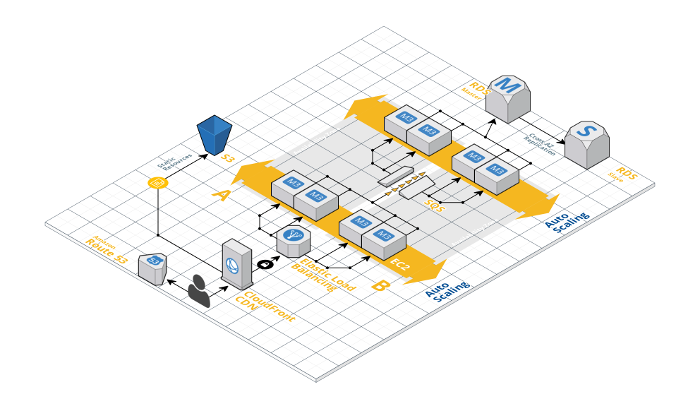
\includegraphics[width=0.8\textwidth]{chapter-2-infrastructure-diagram.png}
    \caption{Contoh gambar}
\end{figure}

\subsubsection{Subsubsubbab}

\blindtext

\begin{table}[h]
    \caption{Tabel random}
    \vspace{0.25cm}
    \begin{center}
        \begin{tabular}{|c|c|c|c|}
            \hline
            Title1 & Title2 & Title3 & Title4  \tabularnewline
            \hline
            1647   & 1.97   & 0.68   & 1.90 \tabularnewline
            2301   & 2.92   & 1.06   & 2.75 \tabularnewline
            2969   & 3.23   & 1.16   & 3.78 \tabularnewline
            3791   & 4.39   & 1.40   & 4.14 \tabularnewline
            4625   & 6.72   & 1.87   & 5.59 \tabularnewline
            \hline
        \end{tabular}
    \end{center}
\end{table}

\section{Menyisipkan Persamaan}

Beberapa contoh menyisipkan persamaan.


\subsection{Contoh Bikin Equation}
\textbf{text tebal} dan ini \emph{miring}, bikin persamaan di baris yang sama, tinggal pake dolar2 $\Psi(\vec{r}_1,...,\vec{r}_N)$, sehingga persamaan Schr\"{o}dinger, terus, persamaan yang dinomeri kayak gini 
%ini contoh bikin persamaan, ..... :D
\begin{equation}
    \left[ \sum_{i}^{N}-\frac{\hbar^2}{2m}\nabla_i^2 + \sum_{i}^{N}V(\vec{r}_i)+ \sum_{i<j}^{N}(\vec{r}_i,\vec{r}_j)\right]\Psi = E\Psi 
\end{equation}

untuk $N$-elektron, dengan $\hat{H}$=Hamiltonian, $E$=Energi total, $\hat{T}$=Energi kinetik, $\hat{V}$=Energi potensial, dan $\hat{U}$=Interaksi ektron-elektron.

\subsection{Bikin Matrix}
Lalalallala.... bikin matrix sekarang, yang ini dikecilin, pake smaller
    {\smaller
        \begin{equation}
            \Psi({\bf r}_1, {\bf r}_2, \cdots {\bf r}_N) = \frac{1}{\sqrt{N!}}\left| \begin{array}{llcl}
                \phi_1({\bf r}_1)     & \phi_2({\bf r}_1)     & \cdots                & \phi_N({\bf r}_1)     \\
                \phi_1({\bf r}_2)     & \phi_2({\bf r}_2)     & \cdots                & \phi_N({\bf r}_2)     \\
                \phi_1({\bf r}_3)     & \phi_2({\bf r}_3)     & \cdots                & \phi_N({\bf r}_3)     \\
                \multicolumn{1}{c}{.} & \multicolumn{1}{c}{.} & \multicolumn{1}{c}{.} & \multicolumn{1}{c}{.} \\
                \multicolumn{1}{c}{.} & \multicolumn{1}{c}{.} & \multicolumn{1}{c}{.} & \multicolumn{1}{c}{.} \\
                \multicolumn{1}{c}{.} & \multicolumn{1}{c}{.} & \multicolumn{1}{c}{.} & \multicolumn{1}{c}{.} \\
                \phi_1({\bf r}_N)     & \phi_2({\bf r}_N)     & \cdots                & \phi_N({\bf r}_N)     \\
            \end{array} \right|
        \end{equation}
    }


% \blankpage
\chapter{Pengembangan \textit{Dataset Trace} I/O NFS dengan Beban Kerja Pelatihan Pembelajaran Mendalam}

\section{Analisis Permasalahan}
Dalam tugas akhir ini terdapat empat permasalahan utama. Pertama, penentuan format dan struktur \textit{dataset trace} I/O NFS. Kedua, pengembangan \textit{tracer} yang digunakan untuk mengembangkan \textit{dataset trace} I/O NFS selama beban pelatihan pembelajaran mendalam dijalankan. Ketiga, pengumpulan dan/atau pengembangan beban kerja pelatihan pembelajaran mendalam yang representatif. Keempat, pelaksanaan analisis terhadap karakteristik I/O yang dihasilkan oleh berbagai strategi \textit{shuffling} (\textit{global, buffered}, dan \textit{bundle}).


\subsection{Penentuan Format dan Struktur \textit{Dataset Trace} I/O NFS}
Dalam pengembangan \textit{dataset trace} I/O NFS, langkah awal yang krusial adalah mengidentifikasi jenis informasi yang perlu direkam. Pemahaman terhadap informasi ini akan menentukan desain dan mekanisme \textit{tracer} yang dikembangkan, khususnya bagaimana \textit{tracer} tersebut mencatat aktivitas I/O selama proses pelatihan model pembelajaran mendalam. Informasi yang dikumpulkan harus mampu merepresentasikan pola akses I/O NFS secara akurat serta relevan untuk mendukung analisis dan pengembangan sistem \textit{cache} dan \textit{prefetching} yang lebih efisien.

Setelah menentukan jenis informasi yang di-\textit{trace}, langkah berikutnya adalah menentukan format \textit{dataset trace} I/O NFS yang dikembangkan. Format tersebut harus memungkinkan peneliti untuk dengan cepat memahami, mengolah, dan mengintegrasikan data \textit{trace} ke dalam berbagai eksperimen atau sistem simulasi mereka. Kemudahan dalam pengembangan dan penggunaan \textit{dataset} sangat penting agar dapat mendukung keberlanjutan riset di bidang \textit{caching} dan \textit{prefetching}.


\subsection{Pengembangan \textit{Tracer}}
Untuk menghasilkan \textit{dataset trace} I/O NFS, perlu dikembangkan sebuah \textit{tracer} yang mampu merekam aktivitas I/O secara spesifik selama beban kerja pelatihan pembelajaran mendalam berlangsung. Prioritas utama dalam pengembangan \textit{tracer} ini adalah integritas data, yang mencakup keakuratan dan kelengkapan informasi yang ditangkap. Meskipun demikian, aspek efisiensi dan \textit{overhead} minimal juga menjadi pertimbangan krusial untuk memastikan proses \textit{tracing} tidak menganggu atau mengubah perilaku asli dari beban kerja pelatihan yang sedang diamati.


\subsection{Beban Kerja Pembelajaran Mendalam}
Langkah awal dalam perancangan beban kerja adalah menentukan jenis tugas pembelajaran mendalam, karena setiap tugas (misalnya, klasifikasi gambar atau deteksi objek) memiliki karakteristik I/O yang unik. Untuk menciptakan skenario yang relevan dengan tantangan komputasi modern, beban kerja dirancang dengan dua karakteristik kunci. Pertama, digunakan \textit{dataset} berukuran besar yang mampu menciptakan I/O \textit{bottleneck} pada lingkungan komputasi umum dengan sumber daya terbatas, seperti Google Colab, di mana keterbatasan memori memaksa sistem untuk terus bergantung pada penyimpanan. Kedua, data diakses secara berulang melalui pelatihan \textit{multi-epoch}, yang merupakan skenario ideal untuk mengukur efektivitas sebuah \textit{cache} melalui \textit{hit ratio}. Kombinasi inilah yang secara konsisten menghasilkan beban kerja terikat I/O: kondisi di mana performa sistem tidak lagi dibatasi oleh kecepatan komputasi, melainkan oleh latensi akses data.

\subsection{Analisis Karakteristik I/O NFS}
Karakteristik I/O pada beban kerja pelatihan pembelajaran mendalam cenderung berbeda dibandingkan dengan aplikasi umum lainnya \parencite{360survey}. Proses pelatihan biasanya melibatkan pembacaan \textit{dataset} berukuran besar secara berulang, sehingga pola akses I/O didominasi oleh operasi pembacaan. Meski demikian, urutan pembacaan dapat bervariasi bergantung pada strategi \textit{shuffling} yang diterapkan. Oleh karena itu, penting untuk mengamati bagaimana variasi strategi \textit{shuffling} ini memengaruhi distribusi dan frekuensi akses data dalam konteks I/O pada sistem NFS.

Dalam konteks \textit{caching} dan \textit{prefetching}, analisis karakteristik I/O perlu memperhatikan aspek \textit{temporal locality} dan \textit{spatial locality} dari pola akses data. \textit{Temporal locality} mengacu pada frekuensi pengaksesan ulang data yang sama dalam rentang waktu yang dekat. Sementara itu, \textit{spatial locality} menggambarkan kecenderungan pengaksesan data secara berdekatan -- misalnya, ketika objek A diakses, objek B yang memiliki asosiasi dengan data A juga cenderung diakses. Karakteristik ini sangat penting bagi efektivitas strategi \textit{caching} karena \textit{cache} bekerja optimal jika pola akses data dapat diprediksi dengan baik. Dengan pemahaman mendalam terhadap karakteristik ini, pengembangan \textit{cache} maupun \textit{prefetcher} NFS yang lebih efisien dan tepat sasaran bagi beban kerja pelatihan pembelajaran mendalam dapat diwujudkan.

\section{Analisis Solusi}

\subsection{Penentuan Format dan Struktur \textit{Dataset Trace} I/O NFS}
Untuk merancang format \textit{dataset trace} yang efektif, langkah pertama adalah mengkaji struktur \textit{trace} yang umum digunakan dalam riset strategi \textit{caching}. Analisis difokuskan pada \textit{trace} yang memfokuskan pada pengaksesan I/O untuk mengidentifikasi informasi fundamental yang relevan. Dari kajian ini, ditemukan bahwa salah satu repositori rujukan utama dalam riset \textit{caching} modern adalah \texttt{twemcacheWorkload/cacheDatasets} yang dikurasi oleh Yang dkk. Repositori ini telah menjadi dasar bagi berbagai riset terkemuka seperti 3L-Cache \parencite{3L-Cache}, Baleen \parencite{Baleen}, dan GL-Cache \parencite{GL-Cache}, yang menunjukkan validitas dan relevansi formatnya.

Berdasarkan dokumen README repositori tersebut, setiap entri \textit{trace} mencakup empat informasi utama, yaitu:
\begin{enumerate}
    \item \texttt{timestamp}: Waktu relatif (dalam UNIX \textit{epoch}) ketika sebuah permintaan I/O terhadap objek terjadi
    \item \texttt{obj\_id}: ID unik yang merepresentasikan setiap objek yang diakses
    \item \texttt{obj\_size}: Ukuran total dari objek yang sedang diakses dalam satuan byte
    \item \texttt{next\_access\_vtime} (opsional): Informasi prediktif mengenai waktu akses berikutnya terhadap objek yang sedang diakses
\end{enumerate}

Berdasarkan analisis tersebut, ditetapkan struktur data untuk \textit{dataset trace} I/O NFS yang dihasilkan. Diadopsi tiga informasi utama dari rujukan, yaitu: \texttt{timestamp}, \texttt{obj\_id}, dan \texttt{obj\_size}. Informasi \texttt{next\_access\_vtime} tidak diimplementasikan, karena proses \textit{tracing} dilakukan secara sinkron bersamaan dengan beban kerja pelatihan sehingga informasi akses di masa depan tidak tersedia.

Untuk keperluan validasi dan analisis \textit{overhead}, proses \textit{tracing} juga akan merekam dua informasi temporer: \texttt{obj\_name} dan \texttt{latency}. Informasi \texttt{obj\_name} digunakan untuk memvalidasi \texttt{obj\_id} telah dipetakan dengan benar dengan \texttt{obj\_size} yang tepat pula. Informasi \texttt{latency} digunakan untuk mengukur dampak performa dari \textit{tracer}. Setelah validasi selesai, kedua informasi temporer ini dihapus. Dengan demikian, struktur akhir dari \textit{dataset trace} I/O NFS yang dihasilkan hanya akan terdiri atas tiga informasi: \texttt{timestamp}, \texttt{obj\_id}, dan \texttt{obj\_size}.

Analisis lebih lanjut pada \textit{dataset} yang dikurasi oleh Yang dkk. menunjukkan bahwa \textit{trace} disimpan dalam format \texttt{oracleGeneral.zst}. Format ini, menurut dokumentasi \texttt{libCacheSim} (sebuah \textit{simulator cache} yang umum digunakan dengan \textit{dataset} tersebut), menawarkan keunggulan performa yang signifikan. Berkas dalam format ini dapat dibaca hingga 10 kali lebih cepat dan menggunakan memori yang lebih sedikit dibandingkan format lainnya seperti \textit{Comma-Separated Values} (CSV) maupun .txt. Berdasarkan pertimbangan kemudahan analisis dan efisiensi simulasi, diputuskan format dari \textit{dataset trace} I/O NFS yang dihasilkan pada tugas akhir ini adalah CSV (untuk kemudahan inspeksi dan analisis data) dan \texttt{oracleGeneral.zst} (untuk kompatibilitas dan performa tinggi saat digunakan oleh peneliti dalam \texttt{libCacheSim}).

\subsection{Pengembangan \textit{Tracer}}
\label{sec:pengembangan_tracer}

\textit{Tracer} untuk tugas akhir ini dikembangkan berbasis \texttt{bpftrace}. Teknologi ini dipilih karena kemampuannya melakukan \textit{tracing} dengan dampak minimal terhadap \textit{throughput} I/O, terutama jika dibandingkan dengan kakas serupa seperti \texttt{strace} \parencite{TracerFile}. \texttt{bpftrace} memanfaatkan \textit{extended Berkeley Packet Filetr} (eBPF) untuk mengeksekusi \textit{script tracing} secara aman di level \textit{kernel} Linux. Mekanisme ini berbasis \textit{event}, bukan \textit{polling}, sehingga jauh lebih efisien.

TODO: rujuk landasan teori NFS
Fleksibilitas \texttt{bpftrace} dalam memasang \textit{probe} menjadi kunci untuk menangkap data I/O NFS secara komprehensif. Berdasarkan analisis alur data I/O NFS (subbab 2.X), informasi utama seperti \texttt{timestamp}, \texttt{obj\_id}, \texttt{obj\_name}, dan \texttt{obj\_size} diperoleh dengan memasang \textit{probe} pada \texttt{kprobe vfs\_read}. Namun, karena \texttt{vfs\_read} adalah fungsi pada lapisan VFS, \textit{probe} ini akan terpicu oleh semua operasi baca dari berbagai jenis \textit{file system}, tidak hanya NFS. Hal ini menciptakan tantangan, yaitu bagaimana menyaring data agar hanya aktivitas I/O yang relevan degnan NFS yang tercatat.

Untuk mengatasi tantangan tersebut, diterapkan mekanisme penyaringan dengan menambahkan \textit{probe} kedua pada \texttt{tracepoint nfs4\_open\_file}. \textit{Tracepoint} ini secara spesifik akan terpicu setiap kali sebuah berkas dibuka melalui protokol NFSv4. Saat terpicu, ID dari berkas yang dibuka akan disimpan. Selanjutnya, di dalam \textit{probe} \texttt{kprobe vfs\_read}, ditambahkan logika untuk memeriksa apakah ID berkas yang sedang diakses terdapat pada kumpulan ID berkas NFS yang telah disimpan sebelumnya. Dengan demikian, pencatatan data hanya akan dilakukan jika berkas tersebut sebelumnya telah diidentifikasi sebagai berkas NFS. Pendekatan dua \textit{probe} ini memastikan \textit{trace} yang dihasilkan memiliki akurasi tinggi dan relevan secara ekslusif pada pengaksesan berkas NFS. Skrip \texttt{bpftrace} yang digunakan pada tugas akhir ini dapat dilihat pada Lampiran \ref{sec:skripbpf}.

\subsection{Beban Kerja Pembelajaran Mendalam}
\label{sec:bebankerja}

Beban kerja pembelajaran mendalam yang digunakan pada tugas akhir ini ditetapkan sebagai tugas klasifikasi gambar. Tugas ini dipilih karena secara inheren melibatkan \textit{dataset} yang berskala besar yang strukturnya terdiri dari ribuan hingga jutaan berkas gambar individual. Struktur "banyak berkas kecil" seperti ini secara alami menghasilkan pola akses I/O yang sangat intensif dan berulang pada granularitas berkas. \textit{File system} harus secara konstan menangani permintaan untuk setiap gambar, menjadikan skenario ini kasus uji yang ideal untuk menelusuri dan mengoptimalkan performa I/O pada level berkas.

Pola akses ini secara fundamental jika dibandingkan dengan beberapa beban kerja lain, contohnya seperti pelatihan model bahasa pada korpus teks yang besar. Meskipun total ukuran \textit{dataset} teks bisa setara atau bahkan lebih besar, datanya sering kali disimpan dalam sejumlah kecil berkas berukuran masif (misalnya, beberapa arsip data berukuran puluhan GB). Pola akses beberapa berkas raksasa ini cenderung lebih sekuensial dan tidak terlalu membebani operasi metadata \textit{file system}. Oleh karena itu, tantangan I/O yang dihadirkan berbeda dan kurang menonjolkan kebutuhan \textit{caching} pada granularitas berkas individual, yang menjadi fokus utama dalam tugas akhir ini.

\textit{Dataset} pelatihan yang digunakan pada tugas akhir ini adalah FireRisk \parencite{FireRisk}. Pemilihan ini didasarkan pada dua pertimbangan utama. Pertama, FireRisk merupakan \textit{dataset} modern yang dipublikasikan pada tahun 2023, sehingga relevan untuk merepresentasikan beban kerja saat ini. Kedua, jumlah datanya yang lebih terkendali (70.331 gambar) dibandingkan dengan alternatif populer seperti ImageNet-1K (1,28 juta gambar) memungkinkan dilakukannya eksperimen dan analisis secara efisien dengan sumber daya komputasi yang tersedia.

\textit{Dataset} FireRisk diperoleh dari repositori HuggingFace, di mana ia pada awalnya tersedia dalam format Parquet. Format ini, yang mengemas banyak gambar ke dalam satu berkas, tidak sesuai dengan tujuan penelitian ini yang memerlukan \textit{tracing} pada granularitas berkas. Oleh karena itu, dilakukan tahap pra-pemrosesan di mana seluruh gambar diekstraksi ke dalam format PNG. Seluruh berkas gambar ini kemudian ditempatkan pada sebuah \textit{server} dan diakses oleh simpul komputasi melalui protokol NFSv4. Konfigurasi ini memastikan setiap operasi baca selama pelatihan menjadi permintaan I/O melalui NFS, sehingga secara akurat menyimulasikan skenario yang akan dianalisis.

\textit{Dataset} FireRisk tidak menyediakan pemisahan standar antara data pelatihan dan validasi. Untuk dapat menganalisis dan membandingkan dua pola akses I/O yang secara fundamental berbeda -- yaitu beban kerja pelatihan yang diacak dan beban kerja validasi yang sekuensial -- terlebih dahulu dilakukan pemisahan \textit{dataset} menggunakan metode \textit{random sampling}. Pembagian dilakukan dengan perbandingan 80\% untuk data pelatihan dan 20\% untuk data validasi untuk memastikan kedua set data merepresentasikan distribusi data asli secara tidak bias.

Setelah pemisahan, kedua set data tersebut digunakan untuk mensimulasikan dua beban kerja yang kontras. \textit{DataLoader} untuk set pelatihan adakan mengacak urutan gambar pada setiap \textit{epoch}, sehingga menghasilkan pola akses I/O yang acak. Sebaliknya, \textit{DataLoader} untuk set validasi tidak akan melakukan pengacakan, menghasilkan pola akses I/O yang sekuensial. Pemisahan ini memungkinkan dilakukannya analisis kehadiran set validasi terhadap strategi \textit{caching} dan \textit{prefetching}.

Meskipun publikasi asli FireRisk menggunakan 100 \textit{epoch} untuk pelatihan, tugas akhir ini menerapkan dua konfigurasi \textit{epoch} yang berbeda dengan dua tujuan spesifik:
\begin{enumerate}
    \item Tahap Analisis (10 \textit{epoch}): Konfigurasi ini digunakan untuk pengumpulan data yang dianalisis dalam naskah tugas akhir ini. Jumlah \textit{epoch} yang lebih sedikit memungkinkan observasi dan analisis pola I/O yang detail dengan waktu eksekusi yang wajar.
    \item Tahap Generasi \textit{Dataset} (100 \textit{epoch}): Konfigurasi ini digunakan untuk menghasilkan artifak utama dari tugas akhir ini, yaitu \textit{dataset trace} I/O yang komprehensif dan kaya akan pola akses berulang. \textit{Trace} yang lebih panjang ini dirancang untuk dapat digunakan kembali oleh peneliti.
\end{enumerate}

Selain \textit{dataset}, arsitektur model yang digunakan umumnya menjadi komponen penting dalam beban kerja pelatihan. Namun, dalam tugas akhir ini, diambil keputusan metodologis untuk mengecualikan komputasi pelatihan model dan hanya mengukur proses iterasi murni terhadap \textit{dataset}. Keputusan ini didasarkan pada fokus utama tugas akhir, yaitu untuk menghasilkan \textit{dataset trace} I/O NFS dan analisis karakteristik pola pengaksessannya. Meskipun komputasi model dapat memengaruhi karakteristik temporal seperti waktu antar-pengaksesan. Dengan demikian, penyederhanaan ini memungkinan beban kerja pembelajaran mendalam menjadi lebih ringan.

Pendekatan ini divalidasi melalui pengujian awal yang membandingkan skenario iterasi data murni dengan skenario pelatihan penuh. Hasilnya mengonfirmasi bahwa urutan pengaksesan berkas pada kedua skenario adalah identik. Meskipun teramati adanya variasi statistik minor pada waktu antar-pengaksesan, perbedaan temporal ini dianggap berada di luar cakupan tugas akhir. Selain justifikasi fokus penelitian, pendekatan ini juga memberikan keuntungan praktis yang signifikan. Dengan menghilangkan waktu komputasi yang intensif, durasi setiap eksperimen menjadi lebih singkat, sehingga memungkinkan dilakukannya pengujian dengan jumlah konfigurasi yang lebih beragam untuk menghasilkan anlaisis yang lebih komprehensif.

\subsubsection{Implementasi \textit{Buffered Shuffling}}
\begin{sloppypar}
Untuk mendapatkan pola akses I/O dari strategi \textit{buffered shuffling}, diimplementasikan sebuah kelas PyTorch kustom bernama \texttt{HFStyleBufferedShuffleDataset} (implementasi dari kelas ini dapat dilihat pada Lampiran \ref{sec:implementasishuffler}). Kelas ini mewarisi dari kelas dasar \texttt{torch.utils.data.IterableDataset}, yang memungkinkan dikontrolnya secara penuh logika iterasi dan pengacakan data. Implementasi kustom ini merujuk pada dokumentasi resmi HuggingFace \parencite{HuggingFaceIterableDataset} dan diperlukan karena fungsionalitas bawaan dari kakas HuggingFace tidak mendukung \textit{dataset} yang diakses dari jalur \textit{file system}, seperti pada penyimpanan NFS yang digunakan pada tugas akhir ini. Konsep inti dari strategi yang diadopsi adalah penerapan lapisan lapisan pengacakan untuk mencapai keseimbangan antara efisiensi I/O dan keacakan data.
\end{sloppypar}

\begin{figure}[t]
    \centering
    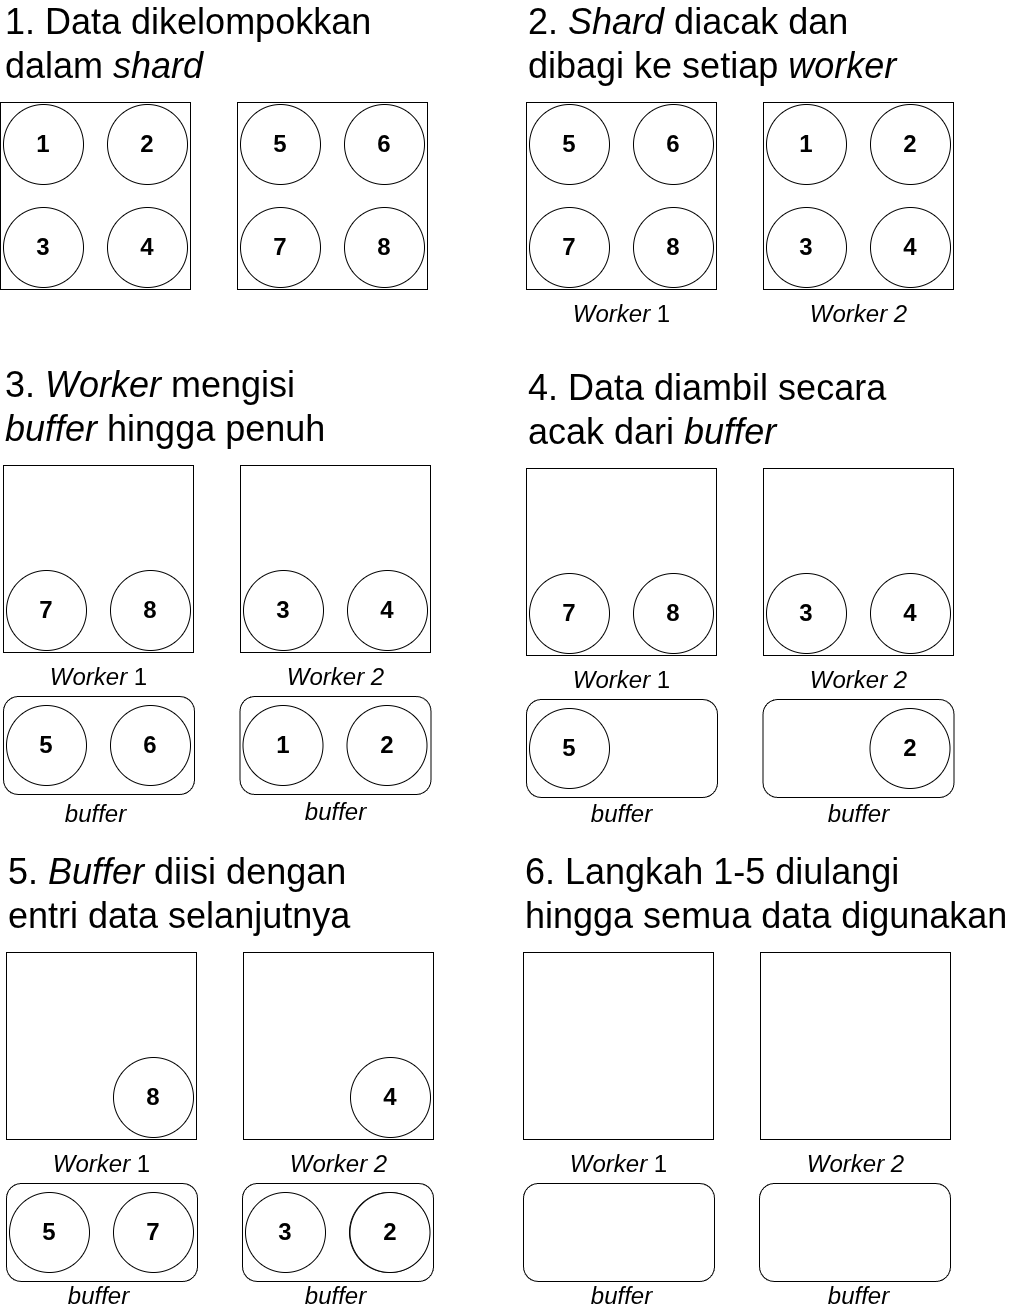
\includegraphics[width=0.7\textwidth]{BufferedShuffling.png}
    \caption{Algoritma \textit{Buffered Shuffling}}
    \label{fig:BufferedShuffling}
\end{figure}

Dua lapisan pengacakan tersebut diimplementasikan sesuai dengan Gambar \ref{fig:BufferedShuffling}. Lapisan pertama adalah pengacakan urutan \textit{shard}: pada awal setiap \textit{epoch}, urutan dari seluruh partisi (\textit{shard}) \textit{dataset} diacak terlebih dahulu. Hal ini memastikan bahwa urutan pemrosesan potongan-potongan besar data akan berbeda pada setiap \textit{epoch}. Lapisan kedua adalah pengacakan di dalam \textit{buffer}, yang bekerja dengan mekanisme yang mirip dengan \textit{reservoir sampling}. Untuk setiap \textit{worker}, sebuah \textit{buffer} dengan ukuran \textit{k} diisi dengan \textit{k} data pertama dari sebuah \textit{shard}. Ketika satu data diminta oleh proses pelatihan, sebuah data akan dipilih secara acak dari \textit{k} data di dalam \textit{buffer}. Posisi yang kosong di dalam \textit{buffer} tersebut kemudian langsung diisi oleh data berikutnya dari \textit{shard} yang sama, menjaga ukuran \textit{buffer} tetap konstan. Proses ini memastikan setiap data yang diberikan ke model merupakan sampel acak dari "jendela" data berukuran \textit{k}.

\subsubsection{Implementasi \textit{Bundle Shuffling}}
Serupa dengan strategi sebelumnya, \textit{bundle shuffling} juga diimplementasikan secara kustom melalui sebuah kelas PyTorch bernama \texttt{BundleShuffleDataset} (implementasi dari kelas ini dapat dilihat pada Lampiran \ref{sec:implementasishuffler}). Kelas ini mewarisi dari \texttt{torch.utils.data.Dataset} dan merujuk pada konsep dari publikasi aslinya \parencite{BundleShuffle}. Namun, dilakukan penyederhanaan pada tugas akhir ini, alih-alih menyebar logika \textit{shuffling} ke dalam tiga komponen (\texttt{Dataset}, \texttt{DataLoader}, dan \texttt{Sampler}) seperti pada implementasi rujukan, seluruh logika dikonsolidasikan ke dalam kelas \texttt{BundleShuffleDataset} untuk mempermudah implementasi.

\begin{figure}[t]
    \centering
    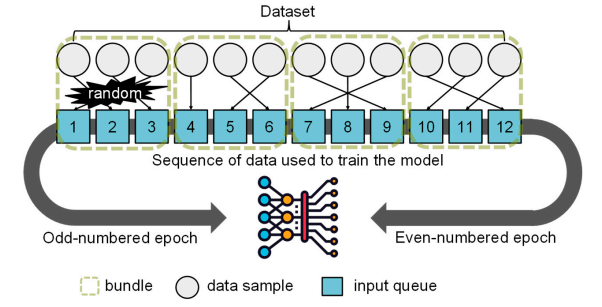
\includegraphics[width=1.0\textwidth]{BundleShuffle.png}
    \caption{Algoritma \textit{Bundle Shuffling}}
    \parencite{BundleShuffle}
    \label{fig:BundleShuffling}
\end{figure}

Mekanisme kerja algoritma ini, yang diilustrasikan pada Gambar \ref{fig:BundleShuffling}, diawali dengan tahap pra-pemrosesan. Pada tahap ini, seluruh data dalam \textit{dataset} dikelompokkan menjadi \textit{M} buah bundel, di mana setiap bundel berisi sejumlah data yang berurutan. Setelah bundel terbentuk, proses pengacakan terjadi pada setiap \textit{epoch} dengan dua karakteristik utama:
\begin{enumerate}
    \item Pengacakan Internal Bundel: Pada awal setiap \textit{epoch}, urutan data di dalam setiap bundel diacak secara individual. Ini memastikan bahwa model menerima data dalam urutan mikro yang berbeda setiap kalinya.
    \item Urutan Akses Bundel Bergantian: Yang menjadi karkateristik unik dari strategi ini adalah urutan pemrosesan bundel yang bersifat deterministik dan bergantian. Pada \textit{epoch} ganjil, bundel diakses secara berurutan dari awal hingga akhir (Bundel 1, 2, ..., \textit{M}). Sebaliknya, pada \textit{epoch} genap, urutan akses dibalik, yaitu dari akhir ke awal (Bundel \textit{M}, \textit{M-1}, \textit{M-2}, ..., 1).
\end{enumerate}

Pola akses bundel bergantian ini menciptakan ketergantungan temporal jangka panjang yang dapat diprediksi. Data-data yang berada di bundel terakhir sebuah \textit{epoch} ganjil akan menjadi data-data pertama yang diakses pada \textit{epoch} genap berikutnya (dan sebaliknya). Karakteristik ini memberikan sinyal prediktif kuat yang berpotensi untuk dieksploitasi oleh strategi \textit{prefetching} yang cerdas.

\subsection{Analisis Karakteristik I/O NFS}
\label{sec:metopenkarakteristik}

Tujuan dari tahap analisis ini adalah untuk mengkarakterisasi beban kerja I/O secara kuantitatif dan kualitatif, yang dihasilkan dari proses penjalanan beban kerja pembelajaran mendalam. Dalam analisis ini, istilah "objek" merujuk pada "berkas" individual. Analisis difokuskan pada bagaimana tiga strategi \textit{shuffling} -- yaitu \textit{global shuffling}, \textit{buffered shuffling}, dan \textit{bundle shuffling} -- memengaruhi pola serta lokalitas akses (\textit{temporal} dan \textit{spatial} locality). Terdapat hipotesis bahwa setiap strategi akan menghasilkan profil lokalitas yang unik; misalnya, \textit{global shuffling} cenderung merusak lokalitas, sementara \textit{bundle shuffling} berpotensi mempertahankannya dalam cakupan \textit{bundle}. Hasil analisis ini akan menjadi landasan untuk merancang strategi \textit{caching} dan \textit{prefetching} yang lebih cerdas dan efisien di masa depan.

\textit{Temporal locality}, atau kecenderungan sebuah berkas diakses kembali dalam waktu dekat, dianalisis menggunakan metrik \textit{reuse distance}. Metrik ini didefinisikan sebagai jumlah operasi akses yang terjadi di antara dua akses beruntun terhadap berkas yang sama. Nilai \textit{reuse distance} yang kecil secara konsisten menandakan \textit{temporal} locality yang tinggi, yang berarti berkas tersebut sangat sering digunakan kembali. Analisis distribusi \textit{reuse distance} sangatlah penting -- jika distribusinya dapat diprediksi, hal ini dapat dieksploitasi. Kebijakan \textit{cache} dapat memprioritaskan berkas dengan prediksi \textit{reuse distance} terkecil, sementara \textit{prefetcher} dapat secara prediktif mengambil berkas yang diperkirakan akan segera diakses kembali.

\textit{Spatial locality}, atau kecenderungan beberapa berkas untuk diakses secara berdekatan dalam waktu, dianalisis menggunakan konsep \textit{lift}. Metrik ini mengukur kekuatan asosiasi antara dua berkas (misalnya, A dan B) dengan menghitung rasio antara probabilitas bersyarat (berkas B diakess setelah berkas A) dengan probabilitas marginal (berkas B diakses secara umum). Nilai \textit{lift} yang lebih besar dari 1 menunjukkan adanya keterkaitan antara akses yang kuat antara A dan B. Dalam konteks \textit{prefetching}, nilai \textit{lift} yang tinggi adalah sinyal jelas untuk melakukan \textit{prefetch} terhadap berkas B setelah A diakses. Selain itu, dalam konteks \textit{caching}, informasi ini dapat dimanfaatkan oleh kebijakan eviksi. Misalnya, saat berkas A diakses, \textit{cache} dapat meningkatkan prioritas berkas B yang berasosiasi kuat (jika sudah ada di \textit{cache}) agar tidak tereviksi, sebagai antisipasi atas akses yang akan datang. Berikut merupakan formula perhitungan nilai \textit{lift}, menurut Tufféry (2011).

\[
\operatorname{lift} = \frac{P(B \mid A)}{P(B)} = \frac{P(B \wedge A)}{P(B) P(A)}
\]

\chapter{Hasil dan Pembahasan}

\section {Lingkungan Eksperimen}

Pengumpulan \textit{dataset} dilakukan pada lingkungan komputasi dan penyimpanan sebagai berikut:

\begin{enumerate}[label=\Alph{enumi}.,topsep=0pt,itemsep=0pt,parsep=0pt]
    \item Klien Pelatihan
        \begin{itemize}[itemsep=0pt, parsep=0pt]
            \item Prosesor: Intel Xeon Silver 4210R (10 \textit{Cores} @ 2.40GHz, 64-bit)
            \item RAM: 80 GB
            \item GPU: Tidak ada
            \item Disk Lokal: 145 GB NVMe SSD
            \item Sistem Operasi: Ubuntu 18.04
            \item Versi Kernel: 5.4.0-150-generic
        \end{itemize}

    \item \textit{Server} Penyimpanan NFS
        \begin{itemize}[itemsep=0pt, parsep=0pt]
            \item Prosesor: Intel Xeon Silver 4110 (16 \textit{Cores} @ 2.10 GH, 64-bit)
            \item RAM: 32 GB
            \item Penyimpanan \textit{Dataset}: RAID 5 dari 3x 6.4 TB
            \item Versi NFS: NFSv4.1
        \end{itemize}
    
    \item Jaringan
        \begin{itemize}[itemsep=0pt, parsep=0pt]
            \item Terhubung melalui ethernet dengan rata-rata \textit{bandwidth} 11,4 Mbps dan rata-rata \textit{Return Trip Time} 0,294 ms
        \end{itemize}

    \item Perangkat Lunak
        \begin{itemize}[itemsep=0pt, parsep=0pt]
            \item Python: 3.8.20
            \item PyTorch: 2.4.1
            \item bpftrace: v0.22.1
        \end{itemize}
\end{enumerate}

\section{Pelaksanaan Eksperimen dan Pengumpulan Data}

\begin{figure}[t]
    \centering
    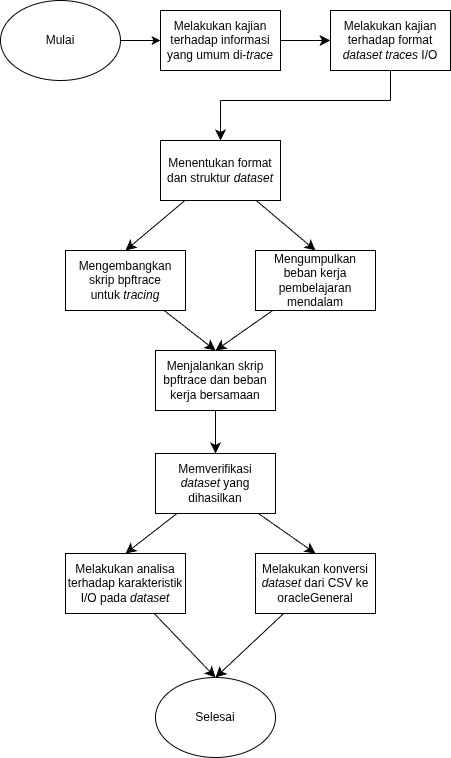
\includegraphics[width=0.6\textwidth]{FlowchartPengerjaan.png}
    \caption{Alur Pengembangan \textit{Dataset}}
    \label{fig:FlowchartPengerjaan}
\end{figure}

Pengembangan \textit{dataset trace} I/O NFS merupakan tujuan utama dari tugas akhir ini. Proses pengembangan \textit{dataset} dilakukan secara sistematis mengikuti alur kerja yang telah diilustraikan pada Gambar \ref{fig:FlowchartPengerjaan}. Sebelum eksekusi, semua komponen telah disiapkan sesuai dengan pembahasan pada Bab III. Sebagai ringkasan, konfigurasi yang digunakan adalah sebagai berikut:
\begin{enumerate}[itemsep=0pt, parsep=0pt]
    \item Informasi pada \textit{Dataset}: Tiga informasi utama yang di-\textit{trace} untuk setiap akses I/O NFS, yaitu \texttt{timestamp}, \texttt{obj\_id}, dan \texttt{obj\_size}, dengan detail seperti yang dirangkum pada Tabel \ref{tab:trace_format}.
    \item Format \textit{Dataset}: \textit{Dataset} final akan disajikan dalam dua format: CSV untuk kemudahan analisis dan oracleGeneral untuk kompatibilitas dengan \textit{simulator} \texttt{libCacheSim}.
    \item \textit{Tracer}: Sebuah skrip \texttt{bpftrace} kustom (dijelaskan pada Subbab \ref{sec:pengembangan_tracer}) digunakan sebagai \textit{tracer}.
    \item Beban Kerja: Beban kerja yang di-\textit{trace} adalah proses iterasi \textit{dataset} pada skenario klasifikasi gambar dengan berbagai strategi \textit{shuffling} (dijelaskan pada Subbab \ref{sec:bebankerja}).
\end{enumerate}

\begin{table}[t]
    \centering
    \caption{Struktur Informasi pada Setiap Entri \textit{Trace}}
    \label{tab:trace_format}
    \begin{tabular}{|l|p{0.6\textwidth}|}
        \hline
        \textbf{Kolom} & \textbf{Deskripsi} \\
        \hline
        \texttt{timestamp} & Waktu relatif saat permintaan I/O terjadi, diukur dalam satuan nanodetik sejak sistem dinyalakan. \\
        \hline
        \texttt{obj\_id}    & ID unik dalam format \textit{integer} yang merepresentasikan setiap berkas yang diakses. \\
        \hline
        \texttt{obj\_size}  & Ukuran total dari berkas yang diakses dalam satuan byte. \\
        \hline
    \end{tabular}
\end{table}

Proses perekaman \textit{trace} dilakukan dengan menjalankan skrip \texttt{bpftrace} dan beban kerja pembelajaran mendalam secara sinkron untuk setiap konfigurasi eksperimen. Keluaran standar dari \texttt{bpftrace}, yang berisi data \textit{trace} baris per baris, dialihkan dan disimpan langsung ke dalam sebuah berkas dengan format \texttt{.csv} menggunakan utilitas \texttt{tee} pada terminal Linux. Pendekatan ini memastikan perekaman data terjadi secara waktu-nyata dengan \textit{overhead} minimal pada proses yang sedang diamati.

Setelah proses perekaman untuk setiap konfigurasi selesai, dilakukan tahap verifikasi data. Proses ini krusial untuk memastikan bahwa \textit{trace} yang dihasilkan bebas dari anomali, lengkap, dan secara akurat merefleksikan aktivitas I/O yang terjadi. Proses validasi dilakukan dengan beberapa pendekatan berikut:
\begin{enumerate}[itemsep=0pt, parsep=0pt]
    \item Konsistensi Waktu: Memastikan nilai pada kolom \texttt{timestamp} selalu terurut menaik.
    \item Konsistensi Ukuran: Memastikan setiap \texttt{obj\_id} yang sama selalu memiliki nilai \texttt{obj\_size} yang identik, karena operasi hanya bersifat baca.
    \item Konsistensi ID: Memastikan setiap \texttt{obj\_id} secara konsisten merujuk pada satu \texttt{obj\_name} yang sama. Untuk tujuan ini, nama berkas juga direkam dalam \textit{trace} mentah namun kemudian dihapus dari \textit{dataset} final untuk menjaga format tetap ringkas.
\end{enumerate}


Setelah sebuah berkas \textit{trace} dinyatakan valid, dua lanxgkah akhir dilakukan. Pertama, untuk tujuan kompatibilitas dengan \textit{simulator} \texttt{libCacheSim}, berkas CSV dikonversi ke format \texttt{oracleGeneral} menggunakan kakas yang disediakan oleh \texttt{libCacheSim}. Kedua, dilakukan analisis karakteristik I/O pada \textit{dataset} CSV menggunakan pendekatan yang telah dijelaskan pada Subbab \ref{sec:metopenkarakteristik}. Dari hasil pengumpulan data ini, dihasilkan serangkaian \textit{dataset trace} I/O NFS yang dirangkum pada Tabel \ref{tab:trace_dataset}.

\begin{table}[t]
    \centering
    \caption{Deskripsi Berkas pada Dataset yang Dihasilkan}
    \label{tab:trace_dataset}
    \begin{tabular}{|l|l|c|c|c|l|}
        \hline
        \thead{\bfseries Nama Berkas} & \thead{\bfseries Dataset} & \thead{\bfseries Kehadiran\\ \bfseries Data Validasi} & \thead{\bfseries Jumlah\\ \bfseries Epoch} & \thead{\bfseries Jumlah\\ \bfseries Worker} & \thead{\bfseries Variasi Shuffling} \\
        \hline
        
        \texttt{\makecell[t]{firerisk\_val\\\_global\_0w}}    & FireRisk & Ada   & 100 & 0  & \textit{Global Shuffling} \\
        \hline
        \texttt{\makecell[t]{firerisk\_val\\\_global\_16w}}   & FireRisk & Ada   & 100 & 16 & \textit{Global Shuffling} \\
        \hline
        \texttt{\makecell[t]{firerisk\\\_global\_0w}}       & FireRisk & Tidak & 100 & 0  & \textit{Global Shuffling} \\
        \hline
        \texttt{\makecell[t]{firerisk\\\_global\_16w}}      & FireRisk & Tidak & 100 & 16 & \textit{Global Shuffling} \\
        \hline
        
        \texttt{\makecell[t]{firerisk\_val\\\_buffer1000\_0w}}  & FireRisk & Ada   & 100 & 0  & \makecell[t]{\textit{Buffered Shuffling}\\(\textit{buffer size} 1000)} \\
        \hline
        \texttt{\makecell[t]{firerisk\_val\\\_buffer1000\_16w}} & FireRisk & Ada   & 100 & 16 & \makecell[t]{\textit{Buffered Shuffling}\\(\textit{buffer size} 1000)} \\
        \hline
        \texttt{\makecell[t]{firerisk\\\_buffer1000\_0w}}      & FireRisk & Tidak & 100 & 0  & \makecell[t]{\textit{Buffered Shuffling}\\(\textit{buffer size} 1000)} \\
        \hline
        \texttt{\makecell[t]{firerisk\\\_buffer1000\_16w}}     & FireRisk & Tidak & 100 & 16 & \makecell[t]{\textit{Buffered Shuffling}\\(\textit{buffer size} 1000)} \\
        \hline

        \texttt{\makecell[t]{firerisk\_val\\\_bundle1000\_0w}}  & FireRisk & Ada   & 100 & 0  & \makecell[t]{\textit{Bundle Shuffling}\\(\textit{bundle size} 1000)} \\
        \hline
        \texttt{\makecell[t]{firerisk\_val\\\_bundle1000\_16w}} & FireRisk & Ada   & 100 & 16 & \makecell[t]{\textit{Bundle Shuffling}\\(\textit{bundle size} 1000)} \\
        \hline
        \texttt{\makecell[t]{firerisk\\\_bundle1000\_0w}}      & FireRisk & Tidak & 100 & 0  & \makecell[t]{\textit{Bundle Shuffling}\\(\textit{bundle size} 1000)} \\
        \hline
        \texttt{\makecell[t]{firerisk\\\_bundle1000\_16w}}     & FireRisk & Tidak & 100 & 16 & \makecell[t]{\textit{Bundle Shuffling}\\(\textit{bundle size} 1000)} \\
        \hline
    \end{tabular}
\end{table}

\section{Karakteristik \textit{Temporal Locality}}
\blindtext

\section{Hasil Pengujian}
\blindtext

\section{Pembahasan}
\blindtext
\chapter{Penutup}

\section{Kesimpulan}
\blindtext

\section{Saran}
\blindtext
%----------------------------------------------------------------%

% Daftar pustaka
\nocite{*}
\printbibliography
\blankpage

% Setting judul lampiran
\titlespacing*{\chapter}{0pt}{0pt}{0pt}
\titlespacing*{\section}{0pt}{0pt}{*1}

% Setting judul anak lampiran
\titleformat*{\section}{\bfseries}

% Index
\appendix
\chapter{Skrip bpftrace yang Digunakan}
\label{sec:skripbpf}

\vspace{1.5pt}

\lstset{
  frame=single,       % Puts a box around the code
  breaklines=true,    % Enables automatic line wrapping
  breakatwhitespace=false, % Prevents breaks only at spaces
  basicstyle=\ttfamily\small % Uses monospaced font for clarity
}

\begin{lstlisting}
tracepoint:nfs4:nfs4_open_file {
 @start[tid] = nsecs;
 @fileinfo[tid] = str(args->name);
 @fileid[tid] = args->fileid;
}

kprobe:vfs_read {
 $ts = nsecs;
 $latency = $ts - @start[tid];
 $filp = (struct file *)arg0;
 $f_path = $filp->f_path;
 $dentry = $f_path.dentry;
 $inode = $dentry->d_inode;
 $size = $inode->i_size;
 printf("%llu,%llu,%s,%llu,%llu\n", $ts, @fileid[tid], @fileinfo[tid], $size, $latency);
 delete(@start[tid]);
 delete(@fileinfo[tid]);
 delete(@fileid[tid]);
}
\end{lstlisting}

\chapter{Implementasi Kelas Kustom \textit{Shuffling}}
\label{sec:implementasishuffler}

\lstset{
  frame=single,
  breaklines=true,
  basicstyle=\ttfamily\small,
  tabsize=4
}

\section{Implementasi \textit{Buffered Shuffling}}
\vspace{1.5pt}
\begin{lstlisting}
class HFStyleBufferedShuffleDataset(IterableDataset):
    def __init__(self, root_dir, transform=None, buffer_size=1024, shuffle=True, seed=None):
        super().__init__()
        self.root_dir = root_dir
        self.transform = transform
        self.buffer_size = buffer_size
        self.shuffle = shuffle
        self.base_seed = seed
        self.epoch = 0
        self._samples = []
        self._class_to_idx = {}
        self._prepare_samples()

    def _prepare_samples(self):
        if not os.path.isdir(self.root_dir):
            raise FileNotFoundError(f"Root directory not found: {self.root_dir}")
        print(f"Scanning '{os.path.basename(self.root_dir)}' to build dataset map...")
        class_names = sorted([d.name for d in os.scandir(self.root_dir) if d.is_dir()])
        self._class_to_idx = {name: i for i, name in enumerate(class_names)}
        for class_name, class_idx in tqdm(self._class_to_idx.items(), desc="Discovering files"):
            class_dir = os.path.join(self.root_dir, class_name)
            for fname in os.listdir(class_dir):
                if fname.lower().endswith((".jpg", ".jpeg", ".png", ".bmp", ".gif")):
                    self._samples.append((os.path.join(class_dir, fname), class_idx))
        print(f"Scan complete. Found {len(self._samples)} images.")

    def __iter__(self):
        rng = random.Random()
        if self.base_seed is not None:
            rng.seed(self.base_seed + self.epoch)
        epoch_samples = list(self._samples)
        if self.shuffle:
            rng.shuffle(epoch_samples)

        worker_info = torch.utils.data.get_worker_info()
        if worker_info is not None:
            num_workers, worker_id = worker_info.num_workers, worker_info.id
            k, m = divmod(len(epoch_samples), num_workers)
            epoch_samples = epoch_samples[worker_id * k + min(worker_id, m):(worker_id + 1) * k + min(worker_id + 1, m)]
        
        return self._data_stream_generator(iter(epoch_samples), rng)

    def _data_stream_generator(self, sample_iterator, rng):
        reservoir_buffer = []
        try:
            for _ in range(self.buffer_size):
                reservoir_buffer.append(next(sample_iterator))
        except StopIteration:
            pass
        if self.shuffle:
            rng.shuffle(reservoir_buffer)
        
        for new_sample in sample_iterator:
            yield_sample = reservoir_buffer.pop(0) if not self.shuffle else reservoir_buffer.pop(rng.randint(0, len(reservoir_buffer) - 1))
            reservoir_buffer.append(new_sample)
            try:
                filepath, label = yield_sample
                img = Image.open(filepath).convert("RGB")
                yield self.transform(img) if self.transform else img, label
            except Exception as e:
                print(f"Error loading {filepath}: {e}. Skipping.")

        if self.shuffle:
            rng.shuffle(reservoir_buffer)
        for remaining_sample in reservoir_buffer:
            try:
                filepath, label = remaining_sample
                img = Image.open(filepath).convert("RGB")
                yield self.transform(img) if self.transform else img, label
            except Exception as e:
                print(f"Error loading {filepath}: {e}. Skipping.")
\end{lstlisting}


\section{Implementasi \textit{Bundle Shuffling}}
\vspace{1.5pt}
\begin{lstlisting}
class BundleShuffleDataset(Dataset):
    def __init__(self, root_dir, transform=None, bundle_size=0, shuffle=True, seed=None):
        self.root_dir = root_dir
        self.transform = transform
        self.bundle_size = bundle_size
        self.shuffle_internal = shuffle
        self.base_seed = seed
        self.current_epoch = -1
        self._samples = []
        self._class_to_idx = {}
        self.base_bundles = None
        self.prepared_epoch_data = []
        self._prepare_samples_and_bundles()

    def _prepare_samples_and_bundles(self):
        if not os.path.isdir(self.root_dir):
            raise FileNotFoundError(f"Root directory not found: {self.root_dir}")
        class_names = sorted([d.name for d in os.scandir(self.root_dir) if d.is_dir()])
        self._class_to_idx = {name: i for i, name in enumerate(class_names)}
        valid_samples = []
        for class_name, class_idx in self._class_to_idx.items():
            class_dir = os.path.join(self.root_dir, class_name)
            for fname in os.listdir(class_dir):
                if fname.lower().endswith((".jpg", ".jpeg", ".png", ".bmp", ".gif")):
                    fpath = os.path.join(class_dir, fname)
                    if os.path.isfile(fpath) and os.path.getsize(fpath) > 0:
                        valid_samples.append((fpath, class_idx))
        self._samples = valid_samples
        self.base_bundles = [self._samples[i:i + self.bundle_size] for i in range(0, len(self._samples), self.bundle_size)] if self._samples else None

    def set_epoch(self, epoch: int):
        if self.current_epoch == epoch and self.prepared_epoch_data:
            return
        self.current_epoch = epoch
        rng = random.Random()
        if self.base_seed is not None:
            rng.seed(self.base_seed + self.current_epoch)
        if self.shuffle_internal:
            if self.base_bundles:
                intra_shuffled_bundles = [list(bundle) for bundle in self.base_bundles]
                for bundle in intra_shuffled_bundles:
                    rng.shuffle(bundle)
                bundles_in_epoch_read_order = intra_shuffled_bundles if self.current_epoch % 2 != 0 else list(reversed(intra_shuffled_bundles))
                self.prepared_epoch_data = [sample for bundle in bundles_in_epoch_read_order for sample in bundle]
            else:
                temp_samples = list(self._samples)
                rng.shuffle(temp_samples)
                self.prepared_epoch_data = temp_samples
        else:
            self.prepared_epoch_data = list(self._samples)

    def __len__(self):
        return len(self._samples)

    def __getitem__(self, index: int):
        if self.current_epoch < 0 or not self.prepared_epoch_data:
            raise RuntimeError("Dataset epoch not set or data not prepared.")
        if not (0 <= index < len(self.prepared_epoch_data)):
            raise IndexError(f"Index {index} out of bounds.")
        filepath, label = self.prepared_epoch_data[index]
        img = Image.open(filepath).convert("RGB")
        return self.transform(img) if self.transform else img, label
\end{lstlisting}


\end{document}
